\chapter{Konzept}

Die Konzeption beschäftigt sich zunächst mit dem Prozess der Feature-Extraktion. Hierfür wird der SIFT Algorithmus nach Lowe genutzt. Folgend wird das Bag of Visual Words Modell näher betrachtet: Es werden auf Basis der Analyse parallele Varianten des Clustering und Histogramm Algorithmus entworfen, die sich zur Ausführung auf Grafikkarten eignen, die CUDA unterstützen. Anschließend wird der geplante Ablauf zum Generieren eines Bag of Visual Word Modells und \textit{Labeling} eines Bildes durch das Modell erläutert.
Abschließend wird auf der Basis der Arbeit von Zhao \cite{aed2016} ein Autoencoder eingeführt, der aus einem HOG Feature-Vektor mit 3042 Komponenten, eine Darstellung des Features in einem Raum mit 36 Dimensionen lernt.

\section{Feature Extraktion}

Die Extraktion der Features ist der erste Schritt zur Erzeugung der Modelle. Das Bag of Visual Words Modell nutzt die vom SIFT-Verfahren erzeugten Feature-Deskriptoren direkt für die weitere Verarbeitung. Der Autoencoder hingegen arbeitet mit den Gradienten der Nachbarschaft der \textit{keypoints} die vom SIFT Feature-Detektor ermittelt wurden. Die Extraktion der Features ist nicht Gegenstand der Parallelisierung bzw. Schwerpunkt dieser Arbeit. Es wird daher auf eine gängige Bibliothek zurückgegriffen, die sich in der Praxis bewährt hat. Sollte sich herausstellen, dass die Feature-Gewinnung einen nicht unerheblichen Teil der Gesamtberechnung ausmacht, kann die Implementierung später noch durch eine parallele bzw. GPU-gestüzte Variante ausgewechselt oder erweitert werden.
Der SIFT Feature-Deskriptor enthält 128 Komponenten und ist so für einen Vergleich nur schwer geeignet: beispielsweise werden bei einem Bild der Größe $320px \times 200px$ bereits 100 bis 1000 Feature-Vektoren generiert. Es werden daher im folgenden zwei Ansätze vorgestellt, welche die Anzahl der Komponenten von Features reduzieren und eine durch Grafikkarten gestützte Berechnung von ähnlichen Bildern ermöglichen.

\section{Ansatz 1: Bag of Visual Words}

In der Analyse wurde bereits sequentielle Varianten des Lloyd und Histogramm Algorithmus vorgestellt und aufgezeigt, an welchen Stellen eine Parallelisierung der Berechnung durch Grafikkarten erfolgen kann. Im Folgenden wird aus diesen Informationen je Algorithmus eine parallele Version für SPMD Prozessoren abgeleitet.
In den beiden nachfolgenden Abschnitten Generierung des Modells und Labeling eines Bildes wird auf den Programmaufbau und -ablauf näher eingegangen. Es werden die wesentlichen Funktionen, ihre Parameter und Aufrufe skizziert.

\subsection{Parellisierung von Llyods Algorithmus}

Der Thread in einem Block mit der \textit{threadId} 0 fungiert hier als Master für die anderen Threads. Die Initialisierung der Cluster mit zufälligen Vektoren aus $v$ wird ebenfalls von diesem übernommen. Die Zuweisung von Vektoren zu Clustern nimmt $\Theta(nk)$ Zeit in Anspruch, wobei $n$ die Anzahl Vektoren und $k$ die Anzahl der Cluster ist. Diese Phase kann parallelisiert werden, in dem pro Feature Vektor ein Thread verwendet wird: Jeder Thread berechnet für seinen Feature Vektor die Distanz zu allen Clusterschwerpunkten und bestimmt den Index des Clusters, der am Nächsten ist. Dieser Prozess ist in Pseudocode in Zeile 6 bis 8 ausgedrückt. Bevor die Cluster aktualisiert werden, müssen die Threads synchronisiert werden: Andernfalls ist nicht garantiert, dass die Berechnung jedes Threads abgeschlossen ist.

\lstset{language=C}
\begin{lstlisting}[mathescape=true]
kmeans_gpu
	if threadId == 0
		$c_{j} = rand(p_{i}) \in P, \: j = 1,...,k, \: c_{j} \neq c_{i} \: \forall i \neq j$
	synchronize threads
	until convergence
		for each $x_{i} \in P_{threadId}$
			$l_{i} = argminD(c_{j}, p_{i})$
		synchronize threads
		if threadId == 0
			for each $p_{i} \in P$
				$c_{l_{i}} = c_{l_{i}} + p_{i}$
				$m_{l_{i}} = m_{l_{i}} + 1$
			for each $c_{j} \in C$
				$c_{j} = \frac{1}{m_{j}} c_{i}$
\end{lstlisting}

\subsection{Parallele Reduzierung von Histogrammen}

Die Berechnung eines Histogramms kann hervorragend parallelisiert werden, da die Operation assoziativ und kommutativ ist: Es spielt keine Rolle in welcher Reihenfolge die Daten abgearbeitet werden bzw. in welcher Reihenfolge die Klassen inkrementiert werden. Wenn das zu beschreibende Histogramm im global Speicher vorliegt, wird die Berechnungsgeschwindigkeit stark reduziert, da viele Threads auf die gleichen Speicheradressen des Histogramms schreibend zugreifen. Damit es nicht zu Lese- / Schreibanomalien kommt, muss das Inkrementieren einer Klasse atomar sein, d.h. zwischen Lese- und Schreibzugriff darf kein anderer Thread auf die Adresse zugreifen. Dies wird in CUDA durch die Operation \textit{atomicAdd} realisiert. Damit die Anzahl an Threads die auf dieselbe Adresse schreiben eingeschränkt wird, arbeitet jeder Block auf einem lokalen Histogramm im \textit{shared memory}. Wenn alle Blöcke ihre lokalen Histogramme berechnet haben, müssen diese noch in das Histogramm im \textit{global memory} kumuliert werden.

\lstset{language=C}
\begin{lstlisting}
__global__
void histogram_kernel (float *buffer, long size, int *histo, int bins) {
	extern __shared__ int *copy[];
	
	if (threadIdx.x < bins) {
		copy[threadIdx.x] = 0;		
	}
	__syncthreads();

	int id = threadIdx.x + blockDim.x * gridDim.x;
	int stride = blockDim.x * gridDim.x;
	
	while (i < stride) {
		int bin = buffer[i] / bins; 
		atomicAdd(&(copy[bin]), 1);
		i += stride;	
	}
	__syncthreads();
	
	if (threadIdx.x < bins) {
		atomicAdd(&(histo[threadIdx.x]), copy[threadIdx.x]);		
	}
}
\end{lstlisting} 

\subsection{Aufbau des Bag of Visual Words Algorithmus}

Das Bag of Visual Words Modell soll zwei Anwendungsfälle unterstützen. Zunächst muss aus einer Menge von Bildern ein Modell generiert werden. Da verschiedene Modelle erstellt werden sollen, müssen diese gespeichert und auch wieder eingelesen werden können. Der Abschnitt Generierung des Modells beschäftigt sich mit einem Entwurf solch eines Systems. Sofern ein Modell generiert wurde, soll es einem Anwender möglich sein ein neues Bild anhand des Modells zu labeln. Dieser Prozess ist in Kapitel Labeling eines Bildes dargestellt.

\subsubsection{Generierung des Modells}

Die Generierung eines Modells kann durch die Funktion \textit{generateModel} gestartet werden. Als Parameter werden der Pfad für die Bilddaten \textit{imageDir}, der Zielpfad \textit{modelPath} und die Anzahl der Cluster \textit{k} erwartet. Der Ablauf der folgenden Funktionsaufrufe ist in Abbildung \ref{img:concept_bovw_1} dargestellt. Im ersten Schritt wird \textit{extractFeatures} aufgerufen, um alle SIFT Features der Bilder, die in \textit{imageDir} enthalten sind, zu extrahieren. Als nächstes werden durch \textit{clusterFeatures} die Features in \textit{k} Cluster gruppiert. Die Berechnung der Cluster, der Distanzen von Features zu Clustern und des Konvergenzkriteriums erfolgt durch die GPU. Als Ergebnis werden die $k$ berechneten Schwerpunkte der Cluster und die Mitgliedschaft der Features zurückgegeben. Abschließend speichert \textit{saveModel} die Cluster unter dem Pfad  \textit{modelPath}/clusters und die Mitgliedschaft unter \textit{modelpath}>/membership. \todo{single extractFeature}

\begin{figure}
	\centering
	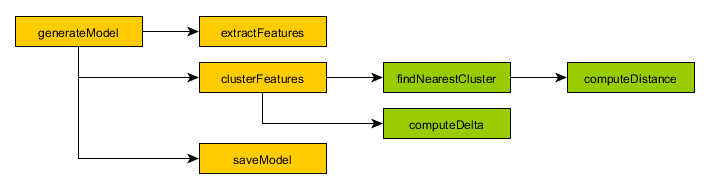
\includegraphics[scale=0.8]{images/concept_bovw_1.png}
	\caption{Funktionen zur Generierung eines Modells}
	\label{img:concept_bovw_1}
\end{figure}

\subsubsection{Labeling eines Bildes}

Sofern ein Modell erstellt wurde, können auf dessen Basis Bilder verglichen werden. In Abbildung \ref{img:concept_bovw_2} sind schematisch die aufeinanderfolgenden Funktionsaufrufe dargestellt. Die Funktion \textit{getImageLabels} wird mit dem Pfad des Modells und des zu vergleichenden Bildes aufgerufen. Das Modell wird durch \textit{readModel} eingelesen und die Clusterschwerpunkte initialisiert. Die SIFT Features werden, wie bei der Generierung, durch \textit{extractFeatures} ermittelt. Die Funktion \textit{selectLabels} berechnet durch \textit{computeFrequencies} das Histogramm der Visual Words aus den Clustern und Features auf der GPU. Auf dieser Basis werden dann die top $num$ Labels ermittelt und zurückgegeben. Hierbei ist die Anzahl der Labels $num$ vom Benutzer festzulegen.

\begin{figure}
	\centering
	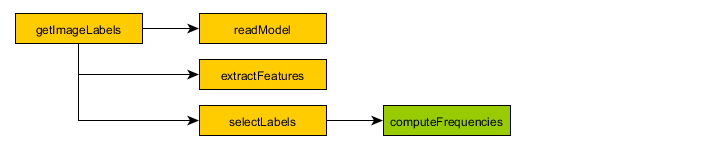
\includegraphics[scale=0.8]{images/concept_bovw_2.png}
	\caption{Funktionen zur Gewinnung von Labels eines Bildes}
	\label{img:concept_bovw_2}
\end{figure}

\section{Ansatz 2: Autoencoder}

In diesem Ansatz wird zur Reduzierung der Dimensionen der Feature-Vektoren ein Stacked Denoising Autoencoder verwendet wie er in der Arbeit von Zhao \cite{aed2016} vorgeschlagen wurde. Der Autoencoder soll eine komprimierte Darstellung der Gradientenvektoren erzielen, die aus den \textit{keypoints} berechnet werden. Hierfür werden Patches der Größe $41 \times 41$ Pixel, zentriert auf den \textit{keypoints}, extrahiert und die Gradienten in horizontale und vertikale Richtung bestimmt. Pro Richtung werden dadurch 1521 Werte erfasst, denn die Gradienten werden in einem Fenster der Größe $39 \times 39$ ermittelt. Dadurch resultiert ein Vektor mit 3042 Elementen für zwei Richtungen. Folglich besitzt der Autoencoder in der Eingabeschicht 3042 Neuronen. Der Encoder des vorgeschlagenen Modells besteht aus fünf Schichten, deren Neuronenanzahl sukzessive reduziert wird, bis schließlich die kleinste Schicht mit 36 Neuronen erreicht wird. Abbildung \ref{img:ae_model} zeigt die Schichten des Encoders sowie Decoders. In der Arbeit von Zhao wurde bereits aufgezeigt, dass der modellierte Autoencoder state of the art Ergebnisse erzielt: Die Ergebnisse des Autoencoders wurden unter verschiedenen Kriterien mit den Ergebnissen der SIFT-PCA und \todo{zweite Methode} Methode verglichen. Dabei erkannte der Autoencoder in fast allen vielen die gleichen Features, jedoch durch einen 36 statt 128 elementigen Feature-Vektor. Theoretisch wird hier also das gleiche Ergebnis in einem Drittel der Zeit ermittelt.

\begin{figure}
	\centering
	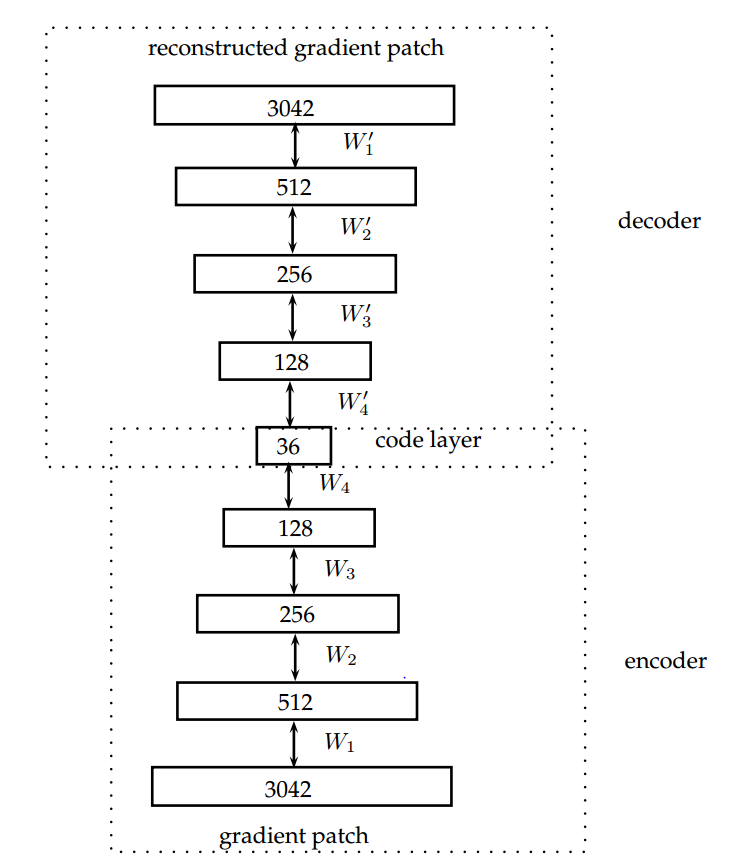
\includegraphics[scale=0.6]{images/ae_model.png}
	\caption{Schichten des verwendeten Autoencoders \cite{aed2016}}
	\label{img:ae_model}
\end{figure}

\subsection{Aufbereitung der Features}

Da der vorgeschlagene Autoencoder nicht direkt mit Bildern arbeitet, sondern Feature-Vektoren, werden die Bilddaten vor der Ausführung entsprechend aufbereitet. Zunächst werden die \textit{keypoints} durch einen SIFT-Detektor ausgewählt. Um die gefundenen \textit{keypoints} wird nun jeweils eine Nachbarschaft der Größe $41 \times 41$ betrachtet. Zum Aufbau des Feature-Vektors werden von diesen Nachbarschaften die Gradienten in horizontale und vertikale Richtung berechnet. Mathematisch entspricht dies einer Konvolution des Ausschnittes mit einem entsprechenden Sobel-Filter. Bei einem Filter mit einem Kernel der Größe $3 \times 3$ entsteht so pro Richtung eine $39 \times 39$ Matrix. Diese werden normalisiert und anschließend zusammen kodiert, sodass der 3042-elementige Feature-Vektor entsteht, der durch den Autoencoder verarbeitet werden kann.
\todo{Sobel}

\subsection{TensorFlow}

TensorFlow ist ein Deep-Learning Framework, dass in Python geschrieben ist. Darüber hinaus gibt aus aber auch Schnittstellen zu anderen Sprachen wie beispielsweise C oder Java. Aus dem Namen leitet sich die bereits die Idee ab, die TensorFlow zugrunde liegt: Ein Tensor ist ein (multidimensionales) Array aus Daten. Diese Tensoren sind mit mathematischen Operationen, den Knoten, miteinander verbunden, sodass die Daten durch die Tensoren und Knoten \grqq fließen\grqq und dabei transformiert werden. Daher eignet sich TensorFlow hervorragend für die Darstellung neuronaler Netze: Die Kanten des Netzes entsprechen den Tensoren, die Neuronen in den Schichten führen mathematische Operationen auf den eingehenden Daten aus und leiten diese weiter an den nächsten Tensor. Die in TensorFlow definierten Modelle lassen sich sowohl auf mehreren CPUs sowie Nvidia GPUs ausführen. Hierfür ist es notwendig, dass auf dem System mindestens CUDA $7.5$ und die cuDNN Bibliothek $4.0$ installiert ist. 
TensorFlow folgt dem sogenannten \glqq lazy\grqq  Programmierparadigma. Dies bedeutet, dass zunächst aus den Definitionen ein Modell aufgebaut wird. Dieses Modell kann durch TensorFlow automatisiert geprüft und visualisiert werden. Im nächsten Schritt werden alle nötigen Variablen initialisiert. Erst durch das Erzeugen und Aufrufen einer \glqq Session\grqq wird das Modell trainiert bzw. auf Testdaten ausgeführt.

\lstset{language=Python}
\begin{lstlisting}
import tensorflow as tf

a = tf.placeholder(tf.int16)
b = tf.placeholder(tf.int16)

addOp = tf.add(a, b)

init = tf.initialize_all_variables()

with tf.Session() as sess:
    sess.run(init)
    print "Addition: %i" % sess.run(addOp, feed_dict={a: 2, b: 3})

sess.close()
\end{lstlisting}